\documentclass[conference]{IEEEtran}
\usepackage{algorithmic}
\usepackage{amsmath,amssymb,amsfonts}
\usepackage{booktabs}
\usepackage{caption}
\usepackage{cite}
\usepackage{dirtree}
\usepackage{fancyhdr}
\usepackage[pdftex]{graphicx}
\usepackage{hyperref}
\usepackage{listings}
\usepackage{pgfplots}
\usepackage{pgfplotstable}
\usepackage{textcomp}
\usepackage{tikz}
\usepackage{url}
\usepackage{xcolor}
\usepackage{xspace}

\usetikzlibrary{positioning, arrows.meta}

\usetikzlibrary{pgfplots.groupplots}

\newcommand{\crayex}{HPE Cray EX\xspace} % standardize name for Cray EX platform
\newcommand{\craympich}{Cray-MPICH\xspace} % standardize name for cray mpich
\newcommand{\stackinator}{Stackinator\xspace} % standardize name the stackinator tool
\newcommand{\spack}{Spack\xspace} % standardize name for spack
\newcommand{\todo}[1]{\textbf{\textcolor{blue}{TODO: #1}}} % add a comment to the article
\newcommand{\assign}[1]{\textbf{\textcolor{blue!20!red}{TODO: #1}}} % add a comment to the article
\newcommand{\hilight}[1]{\textbf{\textcolor{blue!20!red}{#1}}} % add a comment to the article
\newcommand{\tocite}[1]{\textbf{\textcolor{blue!20!red}{[#1]}}} % mark missing citation
\newcommand{\sect}[1]{Section~\ref{#1}\xspace}  % consistent references to sections
\newcommand{\tbl}[1]{Table~\ref{#1}\xspace}  % consistent references to tables
\newcommand{\fig}[1]{Fig.~\ref{#1}\xspace}   % consistent references to figures
\newcommand{\eq}[1]{(\ref{#1})\xspace}   % consistent references to equations
\newcommand{\lst}[1]{\lstinline{#1}\xspace}   % shorthand for inline listing
\newcommand{\libfabric}{libfabric\xspace} % standardize name for cray mpich
\newcommand{\xpmem}{XPMEM\xspace} % standardize name for cray mpich
\newcommand{\openmpi}{OpenMPI\xspace} % standardize name for cray mpich
\newcommand{\nvshmem}{NVSHMEM\xspace} % standardize name for cray mpich
\newcommand{\cufftmp}{cuFFTMp\xspace} % standardize name for cray mpich
\newcommand{\cusolvermp}{cuSOLVERMp\xspace} % standardize name for cray mpich
\newcommand{\miniheader}[1]{\noindent\textsc{#1}\rule{0em}{1.2\baselineskip}\vspace{0.5\baselineskip}}

\definecolor{codegreen}{rgb}{0,0.6,0}
\definecolor{codegray}{rgb}{0.5,0.5,0.5}
\definecolor{codepurple}{rgb}{0.58,0,0.82}
\definecolor{backcolour}{rgb}{0.95,0.95,0.95}

\lstdefinestyle{defaultstyle}{
    backgroundcolor=\color{backcolour},
    commentstyle=\color{codegreen},
    keywordstyle=\color{magenta},
    stringstyle=\color{codepurple},
    basicstyle=\ttfamily\footnotesize,
    breakatwhitespace=false,
    breaklines=true,
    captionpos=b,
    keepspaces=true,
    showspaces=false,
    showstringspaces=false,
    showtabs=false,
    tabsize=2
}

\lstset{style=defaultstyle}

\newcommand\YAMLcolonstyle{\ttfamily\color{magenta}\bfseries\footnotesize}
\newcommand\YAMLkeystyle{\ttfamily\color{blue!50!black}\bfseries\footnotesize}
\newcommand\YAMLvaluestyle{\ttfamily\color{green!50!black}\bfseries\footnotesize}

\makeatletter

% here is a macro expanding to the name of the language
% (handy if you decide to change it further down the road)
\newcommand\language@yaml{yaml}

\expandafter\expandafter\expandafter\lstdefinelanguage
\expandafter{\language@yaml}
{
  keywords={true,false,null,y,n},
  keywordstyle=\color{darkgray}\bfseries,
  basicstyle=\YAMLkeystyle,                                 % assuming a key comes first
  sensitive=false,
  comment=[l]{\#},
  morecomment=[s]{/*}{*/},
%  commentstyle=\color{purple}\ttfamily,
%  stringstyle=\YAMLvaluestyle\ttfamily,
  moredelim=[l][\color{orange}]{\&},
  moredelim=[l][\color{magenta}]{*},
  moredelim=**[il][\YAMLcolonstyle{:}\YAMLvaluestyle]{:},   % switch to value style at :
  morestring=[b]',
  morestring=[b]",
  literate =    {---}{{\ProcessThreeDashes}}3
                {>}{{\textcolor{red}\textgreater}}1     
                {|}{{\textcolor{red}\textbar}}1 
                {\ -\ }{{\mdseries\ -\ }}3,
}

% hyperlink formatting
\hypersetup{
    unicode=true,          % non-Latin characters in Acrobat’s bookmarks
    colorlinks=true,       % colored links
    linkcolor=blue,
    urlcolor=blue
}

\renewcommand\DTstyle{\footnotesize\tt}

\def\BibTeX{{\rm B\kern-.05em{\sc i\kern-.025em b}\kern-.08em
    T\kern-.1667em\lower.7ex\hbox{E}\kern-.125emX}}

\lstset{
    literate={~} {$\sim$}{1}
}
\begin{document}

\title{Modern Software Deployment on a Multi-Tenant Cray-EX System}

\author{
    \IEEEauthorblockN{John Biddiscombe}
    \IEEEauthorblockA{
        \textit{ETH Zurich, Swiss National}\\\textit{Supercomputing Center (CSCS)}\\
        Lugano, Switzerland \\
        john.biddiscombe@cscs.ch}\\
    \IEEEauthorblockN{Ben Cumming}
    \IEEEauthorblockA{
        \textit{ETH Zurich, Swiss National}\\\textit{Supercomputing Center (CSCS)}\\
        Lugano, Switzerland \\
        bcumming@cscs.ch}
    \and
    \IEEEauthorblockN{Jonathan Coles}
    \IEEEauthorblockA{
        \textit{ETH Zurich, Swiss National}\\\textit{Supercomputing Center (CSCS)}\\
        Lugano, Switzerland \\
        jonathan.coles@cscs.ch}\\
    \IEEEauthorblockN{Andreas Fink}
    \IEEEauthorblockA{
        \textit{ETH Zurich, Swiss National}\\\textit{Supercomputing Center (CSCS)}\\
        Lugano, Switzerland \\
        andreas.findk@cscs.ch}
    \and
    \IEEEauthorblockN{Simon Pintarelli}
    \IEEEauthorblockA{
        \textit{ETH Zurich, Swiss National}\\\textit{Supercomputing Center (CSCS)}\\
        Lugano, Switzerland \\
        simon.pintarelli@cscs.ch}\\
    \IEEEauthorblockN{Mikael Simberg}
    \IEEEauthorblockA{
        \textit{ETH Zurich, Swiss National}\\\textit{Supercomputing Center (CSCS)}\\
        Lugano, Switzerland \\
        mikael.simberg@cscs.ch}
}

%\affiliation{%
%  \institution{ETH Zurich, Swiss National Supercomputing Centre (CSCS)}
%  \city{Lugano}
%  \country{Switzerland}
%}

\maketitle

\begin{abstract}
    A key part of HPC centers' service offering is user-facing software -- libraries, tools, applications and programming environments -- tuned for the node and network architecture of the centers' HPC systems.
The teams that maintain and support this software face key challenges: providing a stable software platform for users with long running and fixed project requirements;  providing the latest versions of software for developers; giving full responsibility to build, modify and deploy all levels of the sotware stack to the responsible team (who do not have root access); and reproducible deployment based on GitOps/"as-code" practices.

This paper will discuss how CSCS has addressed these challenges on Alps, by removing the CPE from the configuration of our system, in favour of small independent software environments called uenv, that can be deployed from text-file recipes.
The tool used to build uenv was presented at CUG23.
First, we will discuss adapting Slinghshot-optimised libraries from HPE and NVIDIA (e.g. \cufftmp); the CI/CD pipeline that builds software environments, and deploys them in a container registry; and the command line tools and SLURM plugin that are users' interface to the software environments.

Finally, how the tool is used to provide special use cases such as JupyterHub, and summarise the user and support team experience with the tool -- both positive and negative.

%taking the parts of CPE that we want to provide to users (e.g. cray-mpich), and repackaging them for deployment as isolated, reproducible environments that can be built by CSCS staff and users alike, using pipelines that require no intervention from system administrators, and no modifications to a running system.

%The Cray Programming Environment (CPE) is updated every 6 months, must be installed and modified by system administrators, the provided softare lags behind the latest versions, . Thus updating CPE, and any software that depends on it, can be very disruptive, and is antithetical to addressing our key challenges.

\end{abstract}

\begin{IEEEkeywords}
CPE, spack, squashfs, slurm, gitops
\end{IEEEkeywords}

%%%%%%%%%%%%%%%%%%%%%%%%%%%%%%%%%%%%%%%%%%%%%%%%%%%%%%%%%%%%%%%%%%%%%%%%%%%%%%%
\section{Introduction}
\label{sec:introduction}
A differentiating feature of Alps comparted to other HPE Cray-EX deployments is how multi-tenancy is implemented and supported.
Instead of deploying a single large SLURM cluster, the system is partitioned into non-overlapping SLURM and Kubernetes clusters, each customised for specific use cases and community requirements.
The combination of tenants and use cases requires distributing responsibility for providing and supporting software environments to many individuals and teams inside CSCS.

Ideally software support staff would have end to end responsibility: the ability to install all software as users without interrupting the operation of the system, using automated CI/CD pipelines.
Furthermore, to continue scaling support to more use cases and systems, the tooling and methods used need to:
\begin{itemize}
    \item reduce the dependence of software stacks on the base OS image installed on each tenant
    \item decouple (and simplify) software environments
    \item automate deployment
    \item support users who need to provide their own software stacks.
\end{itemize}

CSCS has found that there is no silver bullet that meets all of these requirements.
For example, HPC containers allow users to bring software stacks built elsewhere, they offer excellent isolation between environments, and container runtimes can inject optimized communication libraries making containerised software resilient to changes to the underlying system.
But supporting containers alone is not sufficient -- we also need to provide software optimised for the target platform, and support users building their own optimized containers.

At CUG 2023 CSCS presented \stackinator~\cite{uenv2023}, a tool for building isolated and reproducible software environments as Squashfs images called uenv, optimized for Cray EX hardware.
This paper focusses on the full end to end process and tooling that CSCS has developed to deploy uenv, how users interact with them, and their impact on support staff.

In \sect{sec:objectives} the requirements discussed above will be enumerated as objectives with measurable aims.
Then the tools and processes used to achieve our objectives will be introduced in three stages: building environments; deploying environments; and the user experience for users of the deployed environments in \sect{sec:methods}.
How CSCS continues to provide CPE as a container, with recipes and lessons learnt for building CPE in a container will be covered in \sect{sec:cpe}.
Finally we will describe some interesting use cases for uenv in \sect{sec:usecases}, and discuss the maintenance overheads and issues with our approach in~\sect{sec:discussion}.

The topics of interest to the CUG audience covered in this paper include:
\begin{itemize}
    \item Providing libraries like OpenMPI and NVIDIA software stack optimized for Slingshot
    \item Reproducible HPC software environments
    \item Using containers to deploy CPE
    \item Modernising the deployment of software on HPC systems
\end{itemize}
Some of the implementation is CSCS-specific, however all of the software and pipelines are in permissibly licensed open source repositories that can be used as is, or used for tips and guidance in developing other sites' solutions.

%%%%%%%%%%%%%%%%%%%%%%%%%%%%%%%%%%%%%%%%%%%%%%%%%%%%%%%%%%%%%%%%%%%%%%%%%%%%%%%

%%%%%%%%%%%%%%%%%%%%%%%%%%%%%%%%%%%%%%%%%%%%%%%%%%%%%%%%%%%%%%%%%%%%%%%%%%%%%%%
\section{Objectives}
\label{sec:objectives}
We first establish concrete objectives that define the requirements for deploying software on HPC systems. These objectives can be used to evaluate the effectiveness of our proposed solutions. The objectives span technical, operational, and organizational aspects of software deployment.

\subsection{Provide optimized software}

Libraries that implement inter-node communication, for example MPI and NCCL, need to be optimized for the Slingshot 11 network in HPE Cray-EX systems.
The method used by \stackinator to install \craympich using Spack~\cite{gamblin:sc15} outside the CPE was demonstrated in~\cite{uenv2023} 

To support all applications, we require similarly robust methods for installing packages like OpenMPI, NCCL, \nvshmem, \cufftmp and \cusolvermp and with libfabric support:
\begin{itemize}
    \item \textbf{aim}: we can deploy key NVIDIA communication libraries on Slingshot 11;
    \item \textbf{aim}: we can deploy OpenMPI with Slingshot 11 support;
    \item \textbf{aim}: build libfabric and CXI from source.
\end{itemize}

\subsection{Gitops deployment}

With GitOps, infrastructure and environments are defined as code in version control systems like Git.
This enables automated, reproducible deployments through CI/CD pipelines, while providing transparency, rollback capabilities, and a single source of truth for the entire system configuration.

We define the following criteria for a GitOps workflow for deploying software on a HPC system:
\begin{itemize}
    \item \textbf{aim}: all software stacks are defined as text file recipes in a git repository;
    \item \textbf{aim}: a CI/CD pipeline builds, tests and deploys uenv images using triggers on the git repository;
    \item \textbf{aim}: each pipeline build deploys unique artifacts;
    \item \textbf{aim}: artifacts can be rebuilt from recipe.
\end{itemize}

\subsection{Decouple environments}

Many use cases on Alps require stable environments that do not change over the duration of multi-year projects,
while others require updated versions of the same environments, or frequent rolling release style deployment to keep pace with rapidly changing software stacks (for example ML/AI and development projects).
%This requires decoupling of software environments, so that new software can be deployed alongside existing software with no side effects, which is summarised with the following aims:
To support all use cases on the same system, we set the following requirements:
\begin{itemize}
    \item \textbf{aim}: existing workflows based are unaffected by releasing new versions of the uenv;
    \item \textbf{aim}: minimise the chance that uenv are ``broken'' by updates to the underlying system, while being able to redeploy them quickly if there is a breaking change;
    \item \textbf{aim}: uenv that provide the latest versions of software (e.g. with pre-releases of cray-mpich or the latest PyTorch version) can be deployed immediately after their release.
\end{itemize}

\subsection{End to end responsibility for software support teams.}

The team responsible for supporting software environments should have full responsibility for its deployment.
Building and deploying software should not require root privileges, modification to the system itself or the involvement of system administrators:
\begin{itemize}
    \item \textbf{aim}: staff who support applications and programming environments should have end to end responsibility;
    \item \textbf{aim}: user communities can manage their own software deployments using the same tools;
    \item \textbf{aim}: individual users can build and share their own uenv images.
\end{itemize}


%%%%%%%%%%%%%%%%%%%%%%%%%%%%%%%%%%%%%%%%%%%%%%%%%%%%%%%%%%%%%%%%%%%%%%%%%%%%%%%

%%%%%%%%%%%%%%%%%%%%%%%%%%%%%%%%%%%%%%%%%%%%%%%%%%%%%%%%%%%%%%%%%%%%%%%%%%%%%%%
\section{The Cray Programming Environment (CPE)}
\label{sec:cpe}
The Cray Programming Environment (CPE) provides a rich software stack: compilers, communication libraries, commonly used scientific libraries and tools.
The CPE is provided by HPE as a collection of RPMs, that CSCS installed using Ansible and deployed to the nodes using the data virtualization service (DVS)\cite{dvs}.

\begin{figure}[htp!]
    \begin{center}
        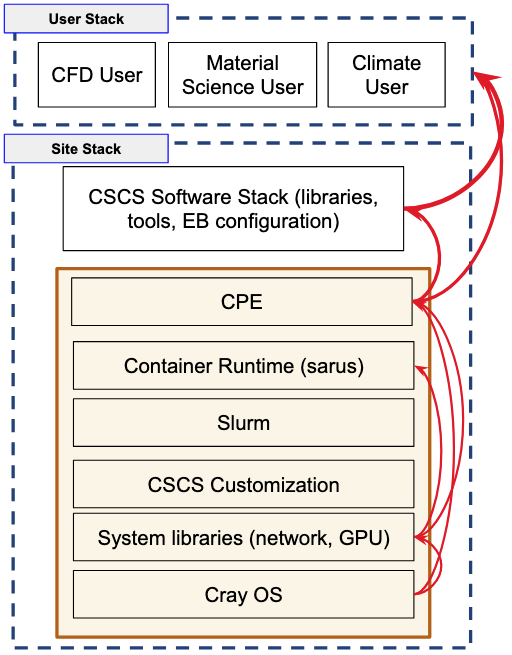
\includegraphics[width=0.4\textwidth]{./images/stack-old.png}
    \end{center}
    \caption{
        The ``standard'' HPE-EX software stack, with the Cray OS, drivers, CPE and site-specific software in the system image, site-provided software installed on a shared file system.
        User-installed software depends on the software layers underneath.
        The red arrows indicate where changes to one layer have a knock on effect on other software layers, requiring rebuilds or reconfiguration.
    }
    \label{fig:cpe-stack}
\end{figure}

To provide additional software to users, HPC centers with HPE Cray-EX systems deploy the CPE, then build additional software using the components it provides -- primarily the compiler wrappers, cray-mpich, CUDA/ROCM and widely-used libraries like FFTw and netcdf.
Centers have developed workflows that use on HPC package management tools like Spack and EasyBuild to build the software, store the configuration in git repositories, and deploy using pipelines with varying levels of automation~\cite{setonix2023,eb2016}.
This additional software is deployed to a shared file system, where it is available for users to use alongside the CPE, as illustrated in~\fig{cpe-stack}.

The downside of this approach is that installing a new version of the CPE, which is released every 6 months, is very disruptive:
\begin{itemize}
    \item changes in the CPE often require reconfiguring and rebuilding centre-provided software - the task of updating Spack and EasyBuild to use new locations and versions of CPE software is particularly time consuming;
    \item users who have built upon this foundation are similarly disrupted;
    \item installing the new CPE requires building a new OS image, typically on a test and deploymebnt (TDS) system;
    \item deployment requires rebooting the system.
\end{itemize}
These disruptions are contrary to all of our objectives for software deployment outlined in~\sect{sec:objectives}
% \item Downside: using CPE as a base layer breaks "no root", "no reboot", and "don't break user codes" tenents

This was the main motivation for CSCS persuing alternatives that don't use CPE for software deployment on Alps, that will be

We note that as of the time of writing, CPE is still available through a \lst{cray} module on the Daint cluster on Alps, for users who require it, or are still in the process of transitioning to uenv and containers.
The \lst{cray} module is the only module available to users on Alps when they first log in, and loading it loads the \lst{PrgEnv-cray} meta-module and populates the full set of available modules.

The module has caused confusion for users, because it is the only obvious software installed on the system when the first log in (unless they have read the documentation).
In \sect{sec:cpe-container} we describe how CSCS will continue providing CPE in a container, in order to improve how CPE is deployed, and help users make a more informed decision about their software environment.

%%%%%%%%%%%%%%%%%%%%%%%%%%%%%%%%%%%%%%%%%%%%%%%%%%%%%%%%%%%%%%%%%%%%%%%%%%%%%%%

%%%%%%%%%%%%%%%%%%%%%%%%%%%%%%%%%%%%%%%%%%%%%%%%%%%%%%%%%%%%%%%%%%%%%%%%%%%%%%%
\section{Methods}
\label{sec:methods}
This section presents the components of CSCS's software deployment workflow, following the complete lifecycle from initial software compilation through to end-user interaction.
We examine three key stages: the building of software components with their specific dependencies and optimizations, the deployment mechanisms across diverse computational environments, and the CLI and SLURM tools that provide these environments to users.
%This structured approach allows us to thoroughly address the complexities inherent in managing scientific software on large-scale HPC systems.

%------------------------------------------------------------------------------
\subsection{Building Software: Stackinator}
\label{sec:stackinator}
%------------------------------------------------------------------------------
The  \stackinator tool, that is used to generate squashfs images from a YAML-based recipe, was documented in detail at CUG 2023~\cite{uenv2023}.
The implementation details of \stackinator were covered in that paper, and have not changed materially.
The method used by \stackinator to install \craympich using Spack~\cite{gamblin:sc15} outside the CPE was demonstrated was shown in~\cite{uenv2023}
This approach is used by \stackinator, however it can also be used directly with Spack -- CSCS staff use it to install the most recent versions of \craympich on LUMI.

\todo{add some more color about stackinator: changes since 2023; per-stack spack versioning; site repo; how all this minimises the Spack upgrade pain.}
\subsubsection{Customizing networking}
\label{sec:networking}
Whilst support for \craympich is mature and well tested, we wish to provide enough flexibility to allow further customization of networking libraries such as
\begin{itemize}
    \item linking \craympich to non default versions of Slingshot dependencies
    \item providing support for non-vendor provided MPI implementations such as OpenMPI
    \item allowing custom versions/branches and options for both top level (MPI) and dependent libraries (libfabric, cxi, etc)
\end{itemize}
To support this, we have extended the \lst{network} section of the \stackinator YAML recipe format where users can override the defaults setup by cluster managers. The following extract \ref{fig:openmpi-config} shows how one can customize all aspects of the networking stack using the rich sytax already provided by spack.
\begin{figure}[htp!]
    \lstinputlisting[language=yaml]{code/openmpi.yaml}
    \caption{Specifying a custom developer version of OpenMPI}
    \label{fig:openmpi-config}
\end{figure}
Stackinator, already supports \lst{package.yaml} customizations, which can be used to override other defaults such as \lst{package_attributes} that specify the git repository location etc.

\todo{NVIDIA libraries}

This section will focus on Spack packing for other key libraries that implement inter-node communication -- for example MPI, NCCL and \nvshmem -- need to be optimized for the Slingshot 11 network in HPE Cray-EX systems.

We will focus on three main sets of libraries. The first is building OpenMPI with libfabric support, in order to provide an alternative to \craympich when there are bugs or performance regressions for specific applications, and to support software that is distributed as binaries linked against OpenMPI. The second is how to build the open source libfabric and CXI driver software for Slingshot 11. Finally, we will show how we adapt \cufftmp and \cusolvermp, which are distributed as pre-build binaries for infiniband, to use \nvshmem with libfabric support, which we developed in collaboration with NVIDIA.

Note that while these methods are integrated into Stackinator, they can be used directly by Spack. All Spack packages, scripts and guides will be made available on GitHub for readers to use.


%------------------------------------------------------------------------------
\subsection{Deployment: CI/CD}
\label{sec:cicd}
%------------------------------------------------------------------------------
Alps has five node node types described in \tbl{tab:alps-nodes}, on top of which CSCS creates vClusters\footnote{Versatile software defined cluster}~\cite{vClusters2023}, where each vCluster is a separate SLURM cluster that is customised for a tenant.
As such, the version of SLURM, mounted file systems and software installed in the OS image (including libfabric) can vary between vClusters.

\begin{table*}[!htb]
    \begin{minipage}{0.6\textwidth}
        \centering
        \begin{tabular}{llrrrr}
        \toprule
        uarch   & type         & blades & nodes & CPU sockets & GPU devices \\
        \midrule
        gh200   & NVIDIA GH200 & 1,344   & 2,688  & 10,752      & 10,752      \\
        zen2    & AMD Rome     & 256     & 1,024  & 2,048       & --          \\
        a100    & NVIDIA A100  & 72      & 144    & 144         & 576         \\
        mi300   & AMD MI300A   & 64      & 128    & 512         & 512         \\
        mi200   & AMD MI250x   & 12      & 24     & 24          & 96          \\
        \midrule
        \multicolumn{2}{c}{\textsc{Total}}      & 1,748   & 3,880  & 13,480  & 11,936 \\
        \bottomrule
        \end{tabular}
    \end{minipage}%
    \begin{minipage}{0.4\textwidth}
        \centering
        \begin{tabular}{lll}
        \toprule
        tenant   & vCluster & uarch         \\
        \midrule
            ML      & Clariden & gh200 \\
            ML      & Bristen  & a100 \\
            HPC     & Daint    & gh200 \\
            HPC     & Eiger    & zen2 \\
            Climate & Santis   & gh200  \\
            MetoSwiss & Balfrin   & a100 and zen2  \\
        \bottomrule
        \end{tabular}
    \end{minipage}
    \caption{Alps node types and their specifications (left), and examples of vClusters provided to tenants (right).}
\label{tab:alps-nodes}
\end{table*}

Over the last two years uenv have proven to be portable between vClusters with the same microarchitecture, and we continue to further reduce the dependence on the underlying OS image, which will also help improve long-term stability of software stacks.
However, to deploy a uenv to a vCluster we still require that it be built on a compute node of the target vCluster to avoid the need for cross compilation, and to ensure that dependencies like libfabric and Slurm are correctly handled.

Manually building and deploying uenv images would be tedious and error prone.
We use a CI/CD pipeline 
\begin{itemize}
    \item The uenv image recipes (YAML files) are maintained in a GitHub repository.
    \item Comments on pull requests trigger a pipeline that builds and tests the uenv image: e.g \lst{system=daint;uarch=gh200;uenv=vasp:v6.5.0}
    \item A GitLab runner that launches build and test stages on the target cluster.
    \item A ReFrame test suite that selects the appropriate tests to run after building the uenv.
\end{itemize}

\todo{expand the points below. Provide an example of the oras commands used to push, pull and attach meta data}

The build pipeline generates two artifacts: a squashfs image and image meta data, which are pushed to an on-premises container registry.
The registry is provided by JFrog\footnote{\href{https://jfrog.com}{\lst{jfrog.com}}}, and Oras\footnote{\href{https://oras.land}{\lst{oras.land}}} is used to push and pull images, so any DockerHub API compatible registry would work.
The images are stored in a \lst{build} namespace, with a tag that corresponds to the unique id of the CI/CD job that built the image, for example:
\begin{lstlisting}
jfrog.svc.cscs.ch/uenv/build/daint/gh200/vasp/v6.5.0:1631426005
\end{lstlisting}

The final deployment is manual, because we find that it is often necessary to first perform additional testing such as providing the image to selected users for validation.
Deployment is performed using the CLI tool (see \sect{sec:cli}):
\begin{lstlisting}
uenv image copy build::vasp:1631426005 \
                deploy::vasp/v6.5.0:v1@daint
\end{lstlisting}
Once deployed, the image is available for users to pull and run.

Users can also use the same build pipeline to build their own uenv from a recipe from anywhere on the CSCS network:
\begin{lstlisting}
> uenv build myapp/v1.2@daint%gh200 <recipe-path>
Log         : https://cicd-ext-mw.cscs.ch/ci/uenv/
build?image=cu3upvpoag1s73eo3n80-3690753405420143
Status      : submitted

Destination
Registry    : jfrog.svc.cscs.ch/uenv
Namespace   : service
Label       : myapp/v1.2:1626811672@daint%gh200
\end{lstlisting}
where \lst{recipe-path} is the YAML recipe.
The link can be used to check the status of the image, and once the image has been built the user can pull it:
\begin{lstlisting}
uenv image pull service::myapp/v1.2:1626811672
\end{lstlisting}




%------------------------------------------------------------------------------
\subsection{User Experience: CLI and SLURM}
\label{sec:cli}
%------------------------------------------------------------------------------
A command line tool called \emph{uenv} is the main interface for uenv users, alongside the SLURM plugin which is documentated in \sect{sec:slurm}.

The uenv tool and SLURM plugin are written in C++, with a library that is used by both, in an open-source GitHub repository\footnote{\href{https://github.com/eth-cscs/uenv2}{\lst{github.com/eth-cscs/uenv2}}}.
The uenv command line tool is a statically-lined executable, and is bundled with the SLURM plugin in a single RPM, for ease of installation.

%---------------------------------------------------
\miniheader{Image Management}
%---------------------------------------------------

\begin{figure}[htp!]
    \dirtree{%
.1 \$SCRATCH/.uenv-images.
.2 index.db.
.2 images.
.3 01edd4\dots76a5ab.
.4 store.squashfs.
.4 env.json.
.4 config.json.
.4 recipe.
.5 \dots.
.4 extra.
.5 reframe.yaml.
.3 e7b0d9\dots47c377.
.4 \dots.
.3 e7e508\dots254742.
.4 \dots.
}


    \caption{The directory layout of a uenv \emph{repository}.}
    \label{fig:repo-path}
\end{figure}

\begin{figure*}[htp!]
    \begin{center}
        \begin{tikzpicture}[
    node distance=5cm and 3cm,
    %every node/.style={font=\sffamily},
    box/.style={draw, thick, minimum width=3.5cm, minimum height=2.5cm, align=center},
    arrow/.style={-{Latex[length=3mm]}, thick}
  ]

  \node[database,label=below:registry,database radius=1cm,database segment height=0.5cm] (rego) {};
  \node[database,label=below:repository,database radius=1cm,database segment height=0.5cm] at (6,-1) (repo) {};
  \node[alice,mirrored,label=below:user, minimum size=1.5cm] at (12,0) (user) {};

  \draw[arrow] (1.2,-0.5)  -- node[above] {image pull} (4.8,-0.5);
  \draw[arrow] (1.2,0.6)   -- node[above] {image find} (11.0,0.6);
  \draw[arrow] (7.5,-0.5)  -- node[above] {image ls} (11.0,-0.5);
  \draw[arrow] (7.5,-1.2)  -- node[above] {image inspect} (11.0,-1.2);
  \draw[arrow] (-1,-1) to[out=120, in=180,looseness=2] (-2,-2)  to[out=0,in=-100,looseness=2] (rego.south west);
  \draw[arrow] (5,-2) to[out=120, in=180,looseness=2] (4,-3) to[out=0,in=-100,looseness=2] (repo.south west);

  \node at (-2,-2.35) {image copy};
  \node at (-2,-2.75) {image delete};

  \node at (4,-3.35) {image add};
  \node at (4,-3.75) {image rm};
\end{tikzpicture}

    \end{center}
    \caption{The uenv image commands are used to manage uenv images in registries and repositories, and to query information about uenv images.}
    \label{fig:uenv-manage}
\end{figure*}

In~\sect{sec:cicd} the CI/CD pipeline that deploys uenv images to a container registry was described.
Users need to download images to local storage before they can use them on a cluster.
The uenv CLI provides a suite of functionality through the \lst{uenv image} command for querying, downloading, and other image management tasks, illustrated in~\fig{fig:uenv-manage}.

There are two locations where uenv images are stored:
\begin{itemize}
    \item \emph{remote}: a \emph{registry} is a container registry from which users can pull images to local storage;
    \item \emph{local}: a \emph{repository} is a directory on a local file system, from which uenv can be run.
\end{itemize}

Local storage for uenv images is a \emph{repository} -- a directory with an SQLite database at the root, and uenv images stored in an images sub-directory.
The database \lst{index.db} at the root of the repository allows for mapping the hash of each uenv to meta data like name, version, micro-architecture and target cluster.
Each image is stored in a path that matches its hash, with the following information:
\begin{itemize}
\item  \lstinline{store.squashfs}: the SquashFS file;
\item  \lstinline{env.json}: information about the mount point, uenv description, and view discriptions (their name, and the environment variable updates that they aplly).
\item  \lstinline{recipe}: the original recipe used to build the image;
\item  \lstinline{extra/reframe.yaml}: description of the testable features the uenv implements, and how to configure the environment to test them.
\end{itemize}

The uenv CLI tool uses the domain-specific language \lst{name/version:tag@system\%uarch} to describe uenv.

Users can query images in the registries and repositories using the \lst{uenv image find} and \lst{uenv images ls} commands respectively, for example the following will search for matching images in the users local repository:
\lstinputlisting[language=bash]{code/uenv-ls.sh}

The \lst{uenv image pull} command is used to pull an image from a remote registry.
The following example searches for all vasp images built for the system daint, pulls one of them, then uses the \lst{image ls} command to show the downloaded image in the local repository:
\lstinputlisting[language=bash]{code/uenv-findpull.sh}

It is possible add and remove images from a local repository using the \lst{uenv image add} and \lst{uenv image rm} commands respectively.

Copying and deleting images in a registry using \lst{uenv image copy} and \lst{uenv image delete} respectively requires permission, which is restricted to the team at CSCS responsible for image deployment.
The \lst{image copy} command is used to deploy by copying images from the \emph{build} namespace (where the CI/CD pipeline pushes them after), to the \emph{deploy} namespace:
\lstinputlisting[language=bash]{code/uenv-deploy.sh}
Note that only one SquashFS image is stored after the two copies in the example above -- each copy creates a new label that is attached to the original SquashFS image.

%---------------------------------------------------
\miniheader{Loading uenv}
%---------------------------------------------------

Before describing how users can load uenv using the uenv CLI, we first define what it means to load a uenv environment.
Loading a uenv provides the software in the \squashfs by mounting the squashfs image and setting environment variables.

The uenv CLI uses the \lst{squashfs-mount} command line utility -- a small \lst{setuid} executable that creates a new mount namespace, mounts the SquashFS file through \lst{libmount}, drops privileges and executes a given command.
The following example starts a bash shell with the Squashfs files \lst{img1.sqfs} and \lst{img2.sqfs} are mounted at \lst{/mnt1} and \lst{/mnt2} respectively:
\lstinputlisting[language=bash]{code/squashfs-mount.sh}
The utility is open source, \href{https://github.com/eth-cscs/squashfs-mount}{available on GitHub} and includes RPMs for installation on Cray EX.

The second part of loading an environment is to set any relevant environment variables.
Each uenv image can provide any number of \emph{views}, which are defined defined in the \lst{meta/env.json} file in the \squashfs file.
Each view is a list of environment varaiables and modifications to make to them, which are applied to the environment variables set in the calling environment.

There are two categories of environment variables:
\begin{itemize}
    \item \emph{Scalar} are environment variables with a single value, for example \lst{CUDA_HOME}, \lst{BOOST_ROOT}, and \lst{TERM}.
        Each scalar variable in a view is a key-value pair, where the key is the variable name, and value is a string or \lst{null}.
        If the value is a string the variable is set (or overriden) to the new value, and if it is \lst{null} the variable is unset.
    \item \emph{Prefix} are environment variables that represent a colon-separted list of paths where the order of paths is significant, for example \lst{PATH}, \lst{LD_LIBRARY_PATH}, and \lst{PKG_CONFIG_PATH}.
        Prefix variables are representated as an ordered set of \emph{updates}, where each update is one of \emph{set}, \emph{prepend}, \emph{append}, \emph{unset}.
\end{itemize}

There are are two views that are automatically generated by Stackinator when the view is built:
\begin{itemize}
    \item\lst{modules}: prepends the module path inside the the uenv to the \lst{MODULE_PATH} environment variable, effectively making modules for packages in the uenv visible.
    \item\lst{spack}: sets environment variables that: point to the Spack configuration for all packages installed inside the uenv; provide the url for the Spack repository; and the branch/commit of Spack that was used.
        Together these variables provide all information required by users to use Spack to build their own software using the packages inside the uenv.
\end{itemize}

Recipe authors can define additional views, that configure the environment similarly to loading a set of modules.
For example, the GROMACS uenv images provide three additional views:
\begin{itemize}
    \item \lst{gromacs}: set all environment variables so that the GROMACS executable is in the path and ready to use.
    \item \lst{plumed}: set all environment variables so that a version of GROMACS with the popular PLUMED plugin is in the path and ready to use.
    \item \lst{develop}: set all environment variables so that all of the libraries, compilers and tools used to build GROMACS are ready to use, without GROMACS, for users who want to build a custom version of GROMACS.
\end{itemize}

%---------------------------------------------------
\miniheader{Using uenv}
%---------------------------------------------------

The uenv CLI provides two methods for using uenv images:
\begin{itemize}
\item\lst{uenv run}: runs a command in the uenv environment before returning to the calling shell.
\item\lst{uenv start}: starts a shell with the uenv environment loaded, for interactive use.
\end{itemize}

The \lst{uenv run} command is the most flexible, because it can be used interactively and in scripts including sbatch scripts.
The examples below show how it can be used to ``wrap'' individual calls in an environment:
\lstinputlisting[language=bash]{code/uenv-run.sh}
In practice there are no performance overheads from wrapping each launch using \lst{uenv run} -- indeed it is much faster than loading and swapping modules then executing software that is installed on a parallel filesystem.
Even when a \squashfs image is stored on Lustre, it is faster and more reliable than accessing the equivalent software stack installed directly on Lustre, because only one file is accessed, and \squashfs efficiently caches files and meta data in memory.

The \lst{uenv start} command is for interactive use cases, for example building software; testing and development; using debuggers and profilers; and using Python or Julia REPLs.
In the next example, the \lst{prgenv-gnu} uenv image is used to create and test a PyTorch virtual environment on a Grace-Hopper node.
The version of Python in the uenv is available through the \lst{default} view:
\lstinputlisting[language=bash]{code/uenv-start.sh}

%---------------------------------------------------
\miniheader{Lessons Learnt}
%---------------------------------------------------

The first version of uenv was written in Python, and was able to modify the calling environment similarly to modules.
For example, the following command would set environment variables for a uenv that was running:
\lstinputlisting[language=bash]{code/uenv-old-view.sh}

A full rewrite of uenv was conducted, based on the lessons learnt from this first version.

The first lesson, which is somewhat subjective, is that Python was not an ideal language for deploying to production for the following reasons:
\begin{itemize}
    \item the call to Python was designed to use Python 3.6 installed as part of SUSE, and had to be isolated;
    \item the project was deployed as a set of directories containing the Python implementating
    \item language features like the lack of type safety and exception-based error handling made implementing a robust, error-free code difficult as the size of the implementation increased.
\end{itemize}

This was simplified greatly by installing a single statically-linked C++ executable, written in C++20 to take advantage of modern language features for error handling, filesystem operations, and sanitizers.

The second lesson was that being able to modify the calling environment over-complicated the implementation, and enabled some bad practices.

In order to modify the calling environment, the \lst{uenv} command was bash function that forwarded the arguments to the Python implementation: \lstinline{echo "$($UENV_CMD $flags "$@")"}, where \lstinline{UENV_CMD} is the path of the implementation.
The implementation would process the arguments, and print a series of shell commands to stdout, which the calling bash function would then exec.
For example, the command \lstinline{uenv view default} might echo the following to stdout:
\lstinputlisting[language=bash]{code/uenv-old-echo.sh}

The wrapper-based implementation made it difficult to debug, required further wrappers inside calls to \lstinline{uenv start} and \lstinline{uenv run}, and made support for different shells difficult -- the original implementation only supported bash.
The new implementation only allows setting views when the uenv is loaded, which is performed by creating a new \lstinline{const char* environ} array that defines the new environment, and forwarding this to \lstinline{execvpe}.
This has the benefits:
\begin{itemize}
    \item the implementation is significantly simplified;
    \item it is shell agnostic - there is no bash-specific code anywhere in the implementation.
\end{itemize}

The final benefit is more subtle: specifying the target environment up front is declarative.
User tickets are easier to debug because the views they are loading are explicitly listed as flags to the uenv call, and all environment modifications are captured in the logs of the \lstinline{uenv start}, \lstinline{uenv run} or SLURM \lstinline{srun --uenv=? --view=?} calls.


%%%%%%%%%%%%%%%%%%%%%%%%%%%%%%%%%%%%%%%%%%%%%%%%%%%%%%%%%%%%%%%%%%%%%%%%%%%%%%%

%%%%%%%%%%%%%%%%%%%%%%%%%%%%%%%%%%%%%%%%%%%%%%%%%%%%%%%%%%%%%%%%%%%%%%%%%%%%%%%
\section{CPE in a Container}
\label{sec:cpe-container}
CSCS provides CPE as an environment on Alps, however installing and updating CPE requires root permission to rebuilding node image and reboot nodes with the new image, and updating the installation of CPE can break user-installed software built on top of the CPE.
This is in opposition to the objective of giving support staff the ability to deploy software stacks without root or interruption to the system.

CSCS provides CPE in a container, because containers can be built using by users with Podman and deployed without modifying the cluster, and the new container does not affect previously deployed CPE containers.
Building CPE containers and deploying them is possible because of two developments:
\begin{itemize}
       \item Alps uses forks of the \href{https://github.com/NVIDIA/enroot}{enroot} container runtime and \href{https://github.com/NVIDIA/pyxis}{Pyxis} Slurm plugin to make using
       \item HPE have improved the modularity of CPE packages, and started releasing them through a new \href{https://cpe.ext.hpe.com/docs/latest/install/installation-guidance-container.html}{RPM repository} that can be used directly in Dockerfiles.
\end{itemize}

%The benefits of deploying CPE in a container include:
%\begin{itemize}
%\item CPE containers can be built, tested and deployed by the support team without root access;
%\item New releases, custom configurations and patched releases of CPE can be deployed without any changes to the underlying system or interruption to service;
%\end{itemize}

With the SLURM integration from Pyxis, starting a job with the CPE is simple, for example starting an interactive shell on a compute node with a specific release of CPE:
\begin{lstlisting}
srun --environment=cpe-24.7 --pty bash
\end{lstlisting}
The container environment is transparent to users, because the Slurm plugin mounts the scratch filesystem so that software built on scratch will be persist between invocations.

The paper will describe the workflow for building containers, and a link to a GitHub repository with DockerFiles use at CSCS, along with ReFrame tests for their deployment.

%%%%%%%%%%%%%%%%%%%%%%%%%%%%%%%%%%%%%%%%%%%%%%%%%%%%%%%%%%%%%%%%%%%%%%%%%%%%%%%

%%%%%%%%%%%%%%%%%%%%%%%%%%%%%%%%%%%%%%%%%%%%%%%%%%%%%%%%%%%%%%%%%%%%%%%%%%%%%%%
\section{Use Cases}
\label{sec:usecases}
%------------------------------------------------------------------------------
\subsection{Standard Environment}
%------------------------------------------------------------------------------

A uenv that provides up to date and modern command line tools, can be mounted on a vCluster.
The package includes editors (e.g. \emph{neovim} and \emph{emacs}), search tools (e.g. \emph{fd} and \emph{ripgrep}), and up to date programming language tools (\emph{lua}, \emph{go}, \emph{rust} and \emph{python}).

The uenv is mounted on the nodes using the equivalent to the following command:
\vfill\eject
\lstinputlisting[language=bash]{./code/manual-uenv-mount.sh}
using a service that can update the mounted image without rebooting the node.

%------------------------------------------------------------------------------
\subsection{JupyterHub}
%------------------------------------------------------------------------------

CSCS provides a JupyterHub web portal for users to access Alps through Jupyter notebooks, which requires the Jupyter software stack installed on the cluster where the session will run.
The approach taken by CSCS is to create a simple \lst{jupyter} uenv that provides only Jupyter and it's requirements.
This uenv is automatically mounted by the JuputerHub service, alongside a uenv selected by the user, which provides the scientific software required.

%------------------------------------------------------------------------------
\subsection{Weather Service Production}
%------------------------------------------------------------------------------

CSCS hosts the operational cluster of The Swiss Weather Service (MeteoSwiss) on Alps -- a system with GPU nodes (4 $\times$ A100 GPU per node) for the weather forecast, and CPU only nodes (2 AMD Xeon CPU per node) for the other tasks in the operational weather forecast pipeline.
The MeteoSwiss pipeline requires two distinct software stacks: an NVHPC stack for their Fortran+OpenACC ICON application; and a GNU toolchain for the other applications in the workflow.
Both stacks are implemented in one uenv, that is mounted permanently at \lst{/mch-environment}.

Due to their strict operational requirements, MCH are naturally very conservative and cautious.
Using uenv has been beneficial because to test a new operational environment the CLI and SLURM plugin can be used to create a session with the new stack mounted on the current stack to perfectly replicate what the permanent deployment would look like.
As we have gained confidence with this approach, we have been able to start splitting the MCH workflow into completely separate environments that are updated at different cadences -- an approach that they would not have agreed to two years ago.


%%%%%%%%%%%%%%%%%%%%%%%%%%%%%%%%%%%%%%%%%%%%%%%%%%%%%%%%%%%%%%%%%%%%%%%%%%%%%%%

%%%%%%%%%%%%%%%%%%%%%%%%%%%%%%%%%%%%%%%%%%%%%%%%%%%%%%%%%%%%%%%%%%%%%%%%%%%%%%%
\section{Discussion}
\label{sec:discussion}
\subsection{The Objectives}
Here we review the original objectives.

\subsubsection{Provide optimised software}

Deployment of key software like MPI, compilers and NVIDIA tools via uenv is on par with or better than CPE.

Our efforts to deploy libfabric, OpenMPI and NVIDIA libraries that are tuned for the system are ongoing, with that provide them available for early testing on the system.
Robust deployment of these components will require the release of Spack 1.0 and improved versioning and release management of the open sourced CXI, Cassini headers and libfabric from HPE.

\subsubsection{Gitops deployment}

The uenv recipes are managed in a GitHub repository, and the tools used by the deployment pipeline are managed in separate GitHub repositories.

The pipeline deploys uenv as discreted artifacts to a container registry that is accessible from the different clusters on Alps.

Finally, each uenv contains the original recipe and other meta data required to rebuild the image at a later date.
Currently the process of rebuilding from a uenv image is quite manual, and is something that will be the focus of future work.

\subsubsection{Decouple environments}

New versions of uenv images can be deployed, without removing or modifying existing environments, so workflows are not affected and can upgrade at their own pace.

This paper did not cover changes to the base OS that is installed on a cluster are managed -- they are tracked in a separate configuration repository.
To date we have only had one breaking change on the system, whereby the libfabric installed as part of the Slingshot host software changed location after an upgrade.
We were able to work around this issue without rebuilding uenv images, however we have the ability to rebuild images in such situations, and our ongoing efforts to install Slinghshot from source inside uenv will further migigate these risks.

Finally, uenv that provide the latest version of cray-mpich are deployed days after it is released, along with uenv that use the pre-release of cray-mpich 9.0 for testing.

\subsection{End to end responsibility for software support teams}

This has been one of the main outcomes of this work -- teams across CSCS are deploying full software stacks with very little central coordination, and with no interaction with system administrators.
See~\sect{discuss-wc} for an example of how users have started deploying their own software stacks.

\subsection{Maintenance overheads}
\label{sec:discuss-staff}

Maintaining the Stackinator tool, the CI pipeline,  and uenv tools is not free -- a core team of two staff performs this work.
One works 75\% on the effort, and the other about 25\%.
CSCS staff actively contribute fixes of their own volition, and contribute to discussions about the architecture and design of the system.
Now that the system is mature, the effort required to maintain it is less than the effort required to develop it.
Overall, the amount of effort required to set up the deployment pipeline and tooling was greater than what was required for the system that it replaced, however this system is more powerful and flexible.

One side effect of this effort is that by decoupling deployment of software environments, a lot more software is being deployed than on the old Piz Daint Cray XC system.
The total amount of effort spent on building and testing software is roughly the same, however more complicated software stacks are being deployed to half a dozen clusters and for a wider range of domains than before.
This leads us to a key observation from CSCS efforts to support multi-tenancy through increased automation and flexibility: the effort required to perform a task like deploying a cluster, building a software stack or adding a dashboard goes down, but the total amount of work stays the same because the number of clusters, software stacks and dashboards will expand to fill capacity.

\subsection{Empowering staff empowers users}
\label{sec:discuss-wc}

One of the objectives was to give staff end-to-end responsibility for software deployed on the system (see~\ref{sec:objective-e2e}).
This was achieved through enabling users to build fully self-contained uenv that include software that was previously installed by system administrators (e.g. \lst{cray-mpich}).
The CI/CD pipeline makes maintaining the recipe, and deploying to different clusters relatively straightforward.

The climate and weather community have started to maintain their own software stacks, by creating recipe repositories and pipelines using the same CI/CD infrastructure.
The registry contains uenv for the production MeteoSwiss environment, and for the software environments used on the climate and weather platform.

The significance of this can't be overstated -- in the past CSCS maintained these challenging software stacks, and the community was often frustrated with forced upgrades or having to iterate with CSCS to define their environment.
It was one of the key aims of the move to multi-tenancy and use-case specific clusters that tenants and communities would take more responsibility for software -- however how this would manifest was not clear.
The current solution was not part of a master-plan, instead it is a happy consequence of the user-first design to empower staff who don't have root.

\subsection{Deploying outside CSCS}
\label{sec:discuss-site}

Much of what has been presented here is site-specific: the on-site container registry and ci/cd infrastructure would be different.
The processes and lessons are transferable, however what we have presented is not a turnkey solution.

The main software tools for building and using uenv are quite easy to get running locally.
Stackinator can be used to build squashfs images, or even to install isolated solftware stacks in a directory on a shared file system.
The uenv CLI tool and SLURM plugin have some site-specific customization related to:
\begin{itemize}
    \item the container registry address and some quirks of dealing with its API;
    \item determining the name of the cluster on which the tool is being used;
    \item determining the username;
    \item and configuring credentials for interacting with the registry.
\end{itemize}
These are implemented in a separate C++ header and implementation file, which can be customised.
Note that these features are only required for interacting with a remote registry: the tools will still function with a local repository.
If there is interest from other sites, this could be refactored to make registry interaction more plug and play.

%%%%%%%%%%%%%%%%%%%%%%%%%%%%%%%%%%%%%%%%%%%%%%%%%%%%%%%%%%%%%%%%%%%%%%%%%%%%%%%

% TODO: before submission, use this to balance the columns on the last page
\vfill\eject

%*************************************************
\bibliographystyle{abbrv}
\bibliography{refs}
%*************************************************

\end{document}

%%% Local Variables:
%%% TeX-engine: default
%%% End:
